\chapter{Second Contribution}
\label{chap:chapter4}
Software to find anomalies works at some level in the system to protect an electronic network from unauthorized users, which maybe insiders as well as outsiders. The task in anomaly detection is to build an algorithm or model which is capable of differentiating between *bad connections*, known as intrusions or attacks, and *good traditional connections*.\newline
A connection may be a sequence of communications protocol packets beginning and ending at some well outlined times, between that information flows to and from a specified address to a target destination address beneath some well-defined protocols. Every connection is labelled as either traditional, or as an attack, with specifically one specific attack kind. Every connection record consists of concerning a hundred bytes.\newline \newline
Attacks make up four main categories: \newline
- DOS: denial-of-service, e.g. syn flood;\newline 
- R2L: unauthorized access from a far off machine, e.g. guesswork password;\newline 
- U2R: unauthorized access to native superuser (root) privileges, e.g., numerous ``buffer overflow'' attacks; \newline
- searching: law agencies investigation and different probing, e.g., port scanning.\newline
\newline
\newline
Almost all novel attacks are square measure of variants of notable attacks and therefore the "signature" of notable attacks may be ample to catch novel variants. supporting this concept, we are going to experiment with a few approaches. We will begin by acting on a reduced data set (the ten percent data set provided). \newline\newline

We will do some exploration of data using Panda library in python. Then we will try to build a model. Our model can simply classify entries into normal or attack. By doing so, we will generalise the model to attack varieties. \newline
\begin{figure}
    \centering
    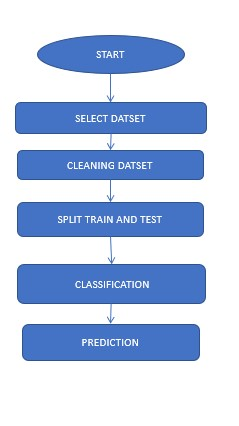
\includegraphics{texfiles/images/flow_diagram.jpg}
    \caption{Flow Diagram}
    \label{fig:flow_diagram}
\end{figure}
However, in our final approach we will use data analytics techniques for anomaly detection. We would like our model to be able to work well with known attack varieties and conjointly to present an approximation of the nearest attack kind. At the start we are going to do agglomeration victimization once more and see if we will beat our previous classification.\newline

\begin{figure}
    \centering
    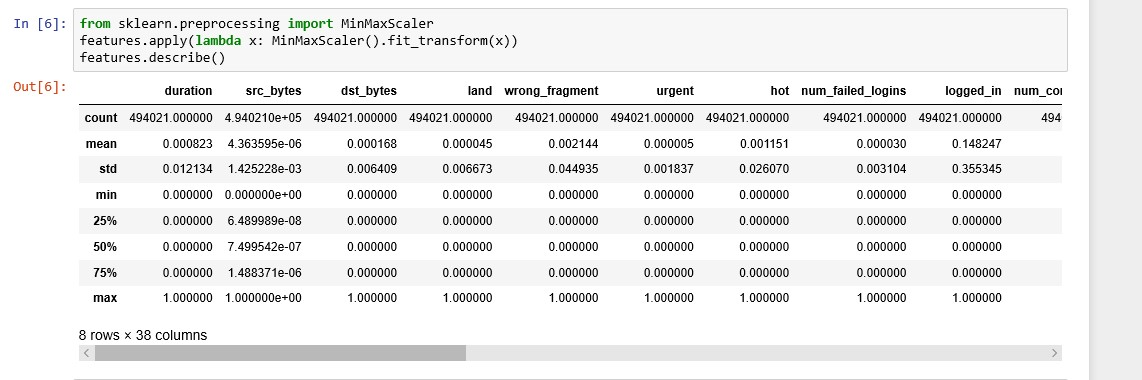
\includegraphics{texfiles/images/feature_extraction_in_code1.jpg}
    \caption{Feature Extraction}
    \label{fig:Feature Extraction}
\end{figure}

\begin{figure}
    \centering
    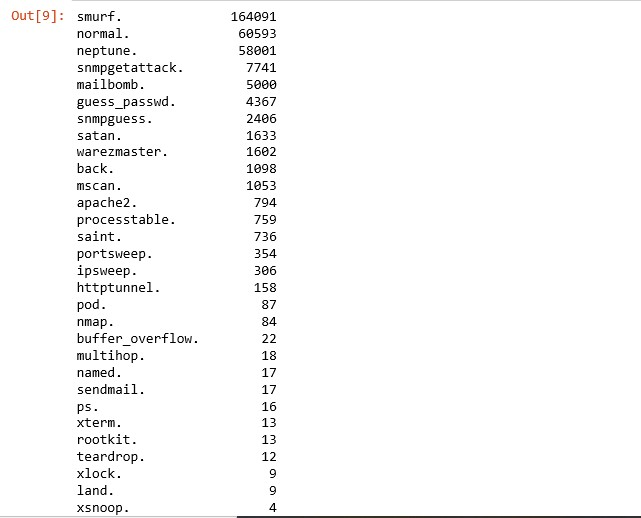
\includegraphics{texfiles/images/number_of_attacks.jpg}
    \caption{Number of Attacks}
    \label{fig:Attack Identification}
\end{figure}
  Visualising information  principal elements
By studying victimization information using principal part analysis, we will cut back the spatial property of our information and plot it into a two-dimensional area. The PCA can capture those dimensions with the most variance, reducing the knowledge loss. 
\textbf{Building a classifier} 
Following the concept that new attack varieties are just like notable varieties, let's begin by attempting a k-nearest neighbours classifier. we have a tendency to should to avoid brute force comparisons within the Nxd area in the least prices. Being n the amount of samples in our information quite , and d the amount of options , we are going to find a possible modelling 
method. Our try our anomaly detection approach within the reduced data set. We are going to begin by doing k-means agglomeration. Once we've got the cluster centre’s, we are going to use them to see the labels of the check information (unlabelled). Based on the idea that new attack varieties can fit previous kind, we are going to be able to sight those. Moreover, something that falls too aloof from any cluster, are thought-about abnormal and thus a potential attack

